% vim: spell spelllang=en:
%! TEX root = **/00-main.tex

% Hierarchical Clustering on original data:

\section{Hierarchical Clustering}%
\label{sec:hierarchical_clustering}

\subsection{Description of data}%
\label{sub:description_data}
% TODO:

% Precise description of the data used (which variables have not been included
% in the analysis, if any, whenever you are using a CURE strategy, provide
% details about eventual sampling performed on data, etc)

We decided to investigate two different hierarchical clustering methods to
identify which one worked best with our data set: Ward's hierarchical method and 
Hierarchical Clustering on Principal Components (HCPC). Ward uses
the whole preprocessed data set while HCPC uses the PCA outcome. None of the
methods required any kind of sampling.

\subsection{Methods, metrics and criteria}

% Clustering method used, metrics and aggregation criteria used (Ward’s method
% is recommended embedded or not in a CURE strategy whenever scaling to big data
% is required, for messy data Gower dissimilarity coefficient to the square is
% recommended )

As mentioned in \ref{sub:description_data}, we explored two different clustering methods.
Ward chooses which two clusters to merge based on the pair of clusters that leads to the
minimum increase in the sum of squared Euclidean distances for the merged cluster. 
On the other hand, HCPC applies the same Ward criterion but on the principal components 
not to the whole data set.


\subsection{Dendogram}

\begin{figure}[H]
    \centering
    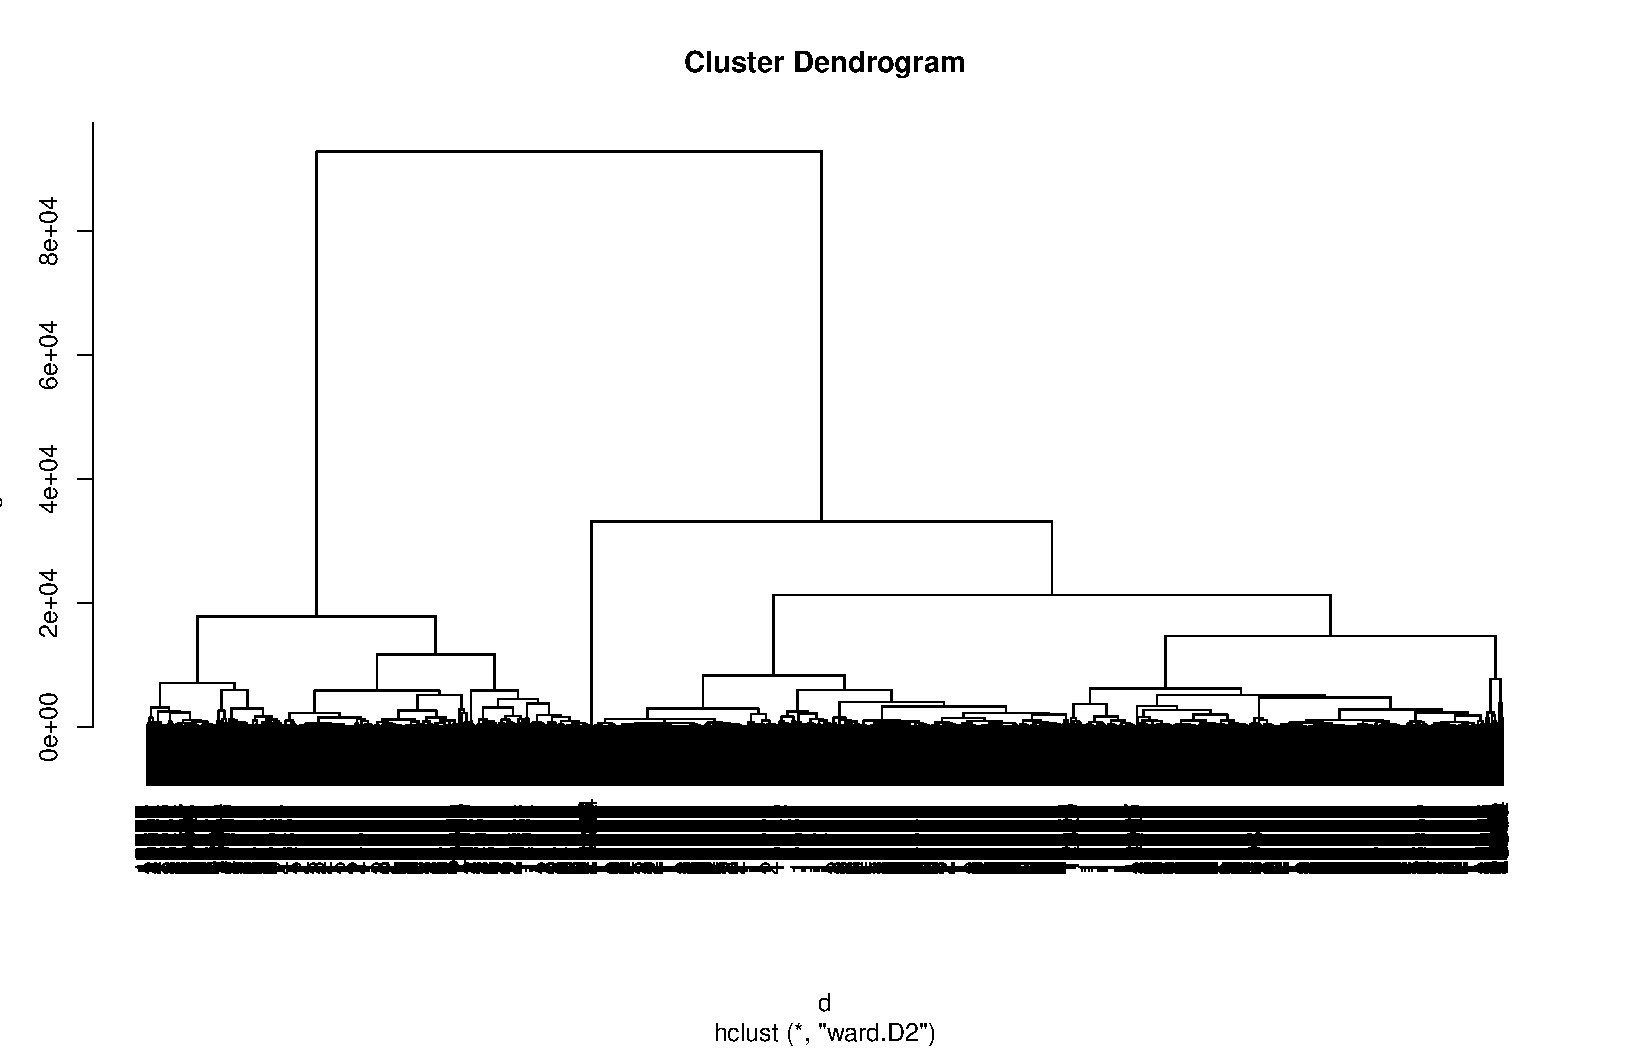
\includegraphics[width=0.8\linewidth]{cluster-dendo-h2}
    \caption{Cluster Dendogram}%
    \label{fig:dendogram-h2}
\end{figure}

\begin{figure}[H]
    \centering
    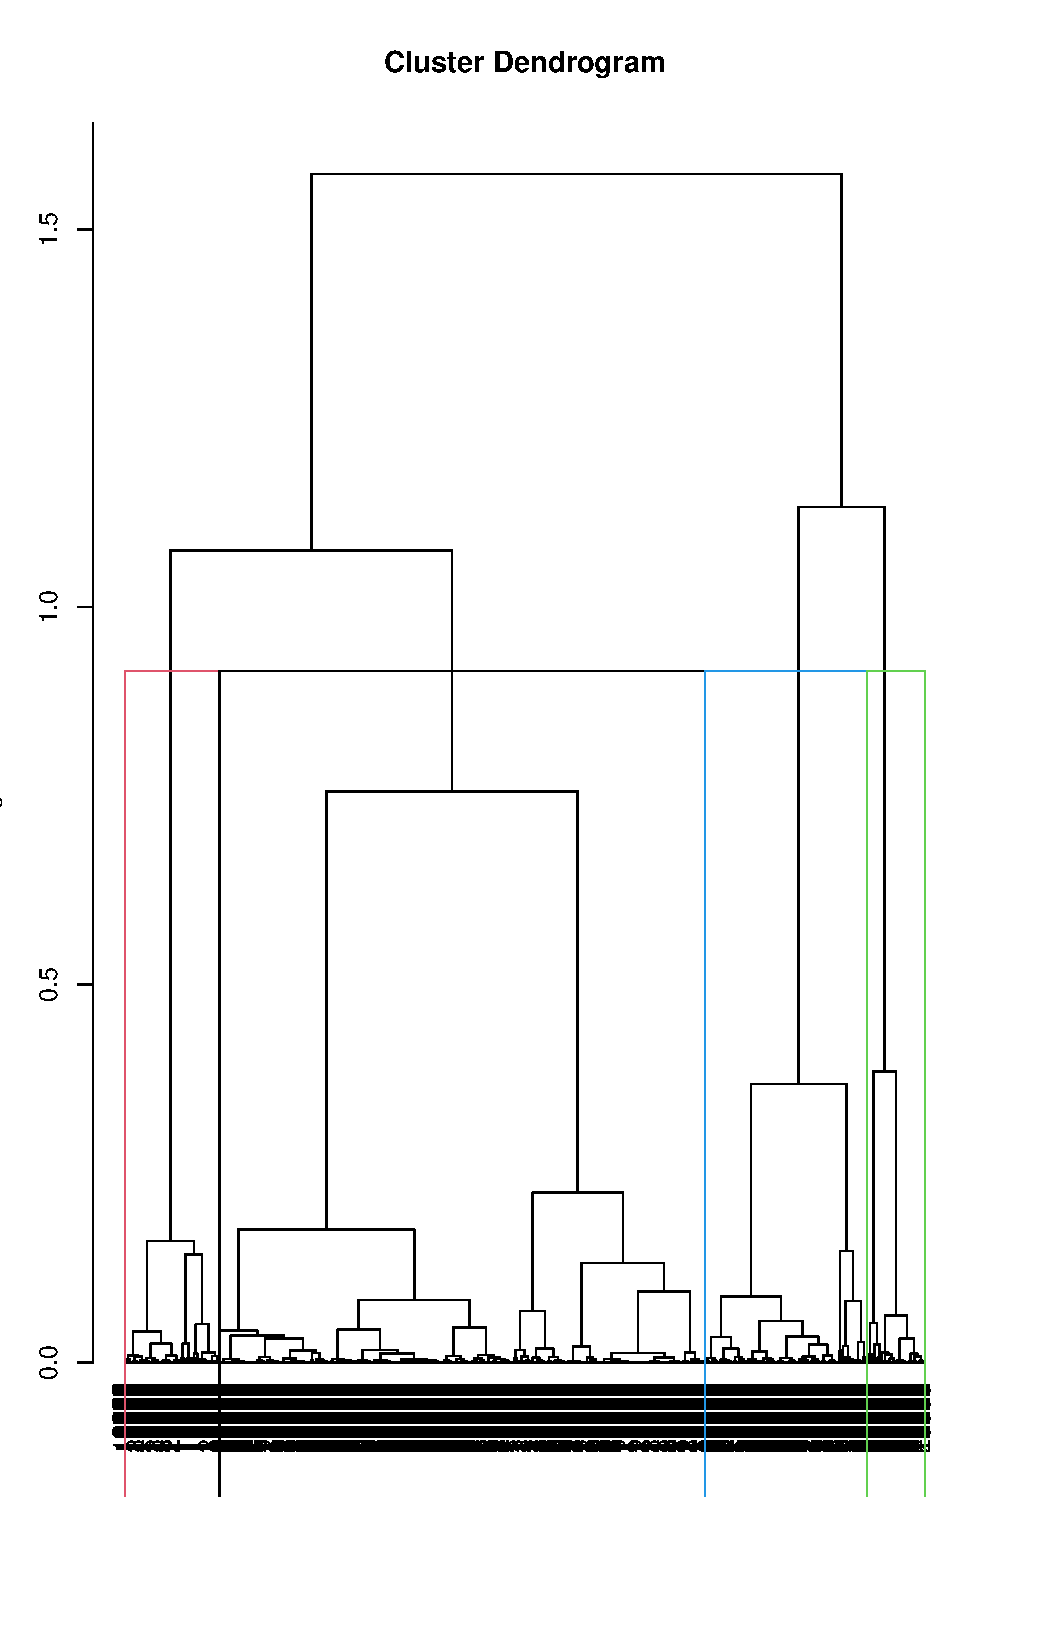
\includegraphics[width=0.8\linewidth]{cluster-dendo-h3}
    \caption{Cluster Dendogram}%
    \label{fig:dendogram-h3}
\end{figure}

\begin{landscape}

\subsection{Dendogram}%
\label{sub:dendogram}

% Resulting Dendrogram (of the total dataset or the sample). USE A SINGLE PAGE
% for it

\begin{figure}[H]
    \centering
    %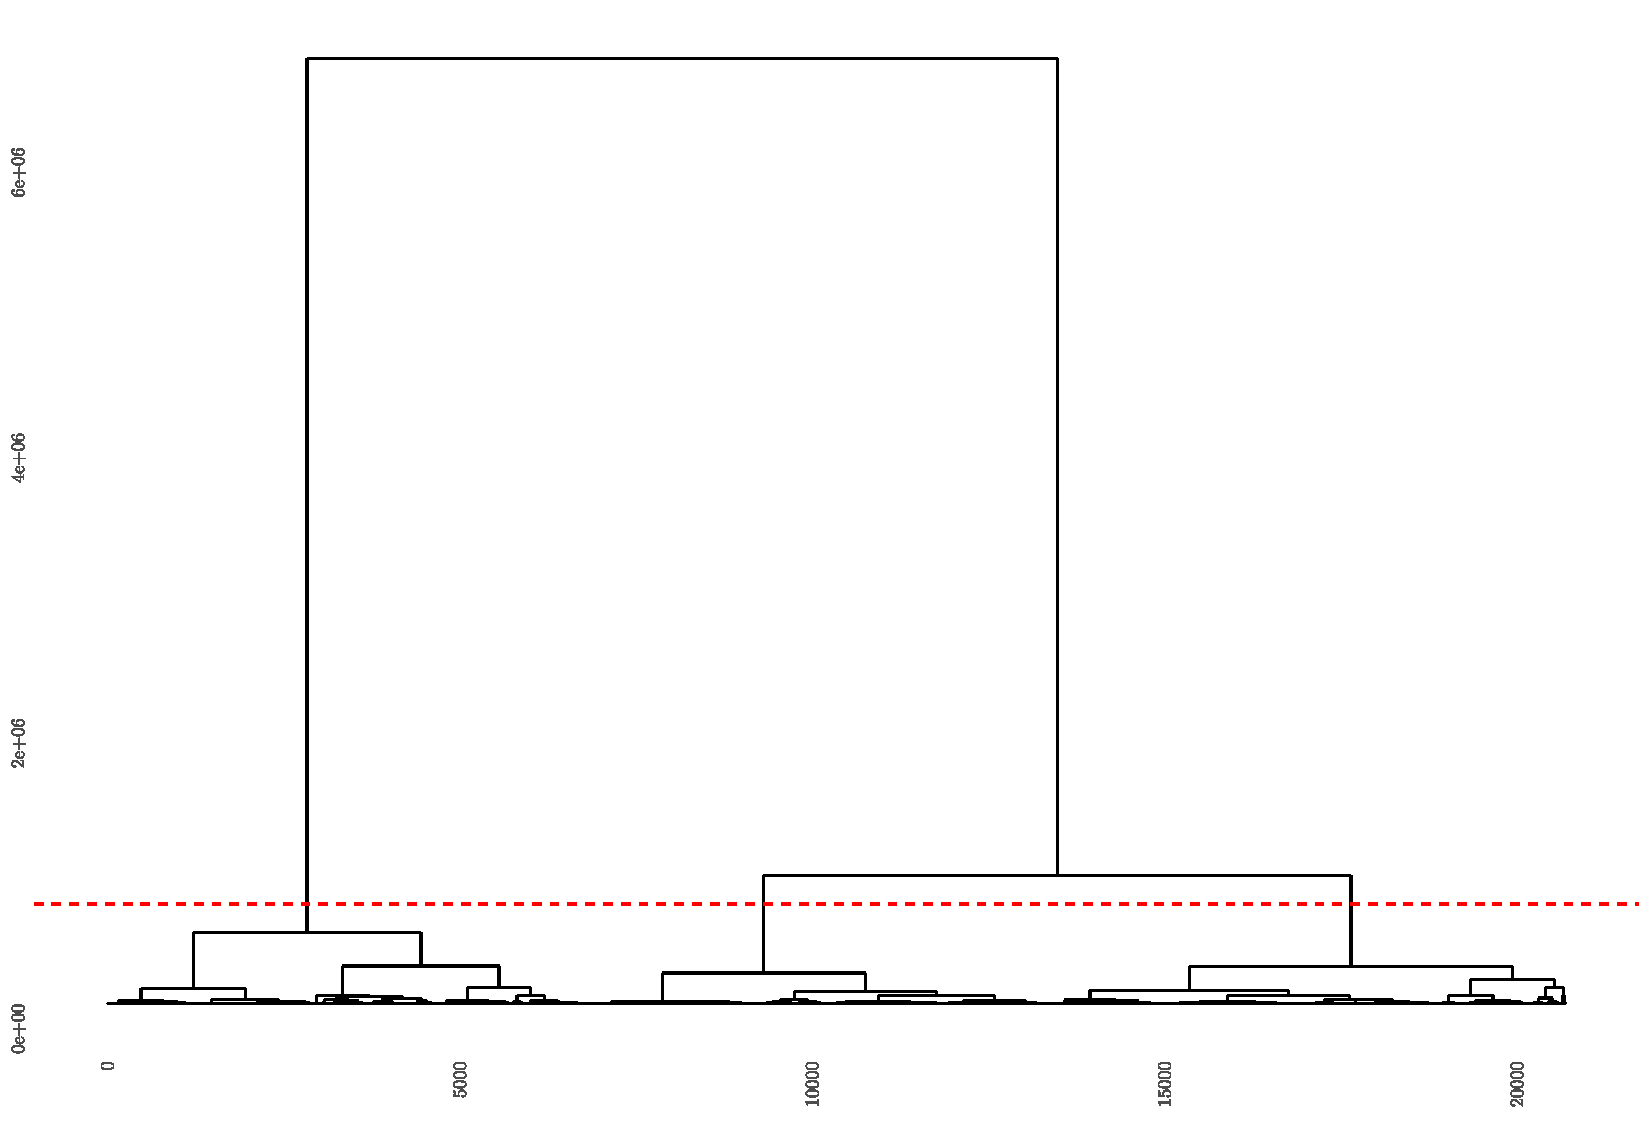
\includegraphics[width=0.8\linewidth]{dendo}
    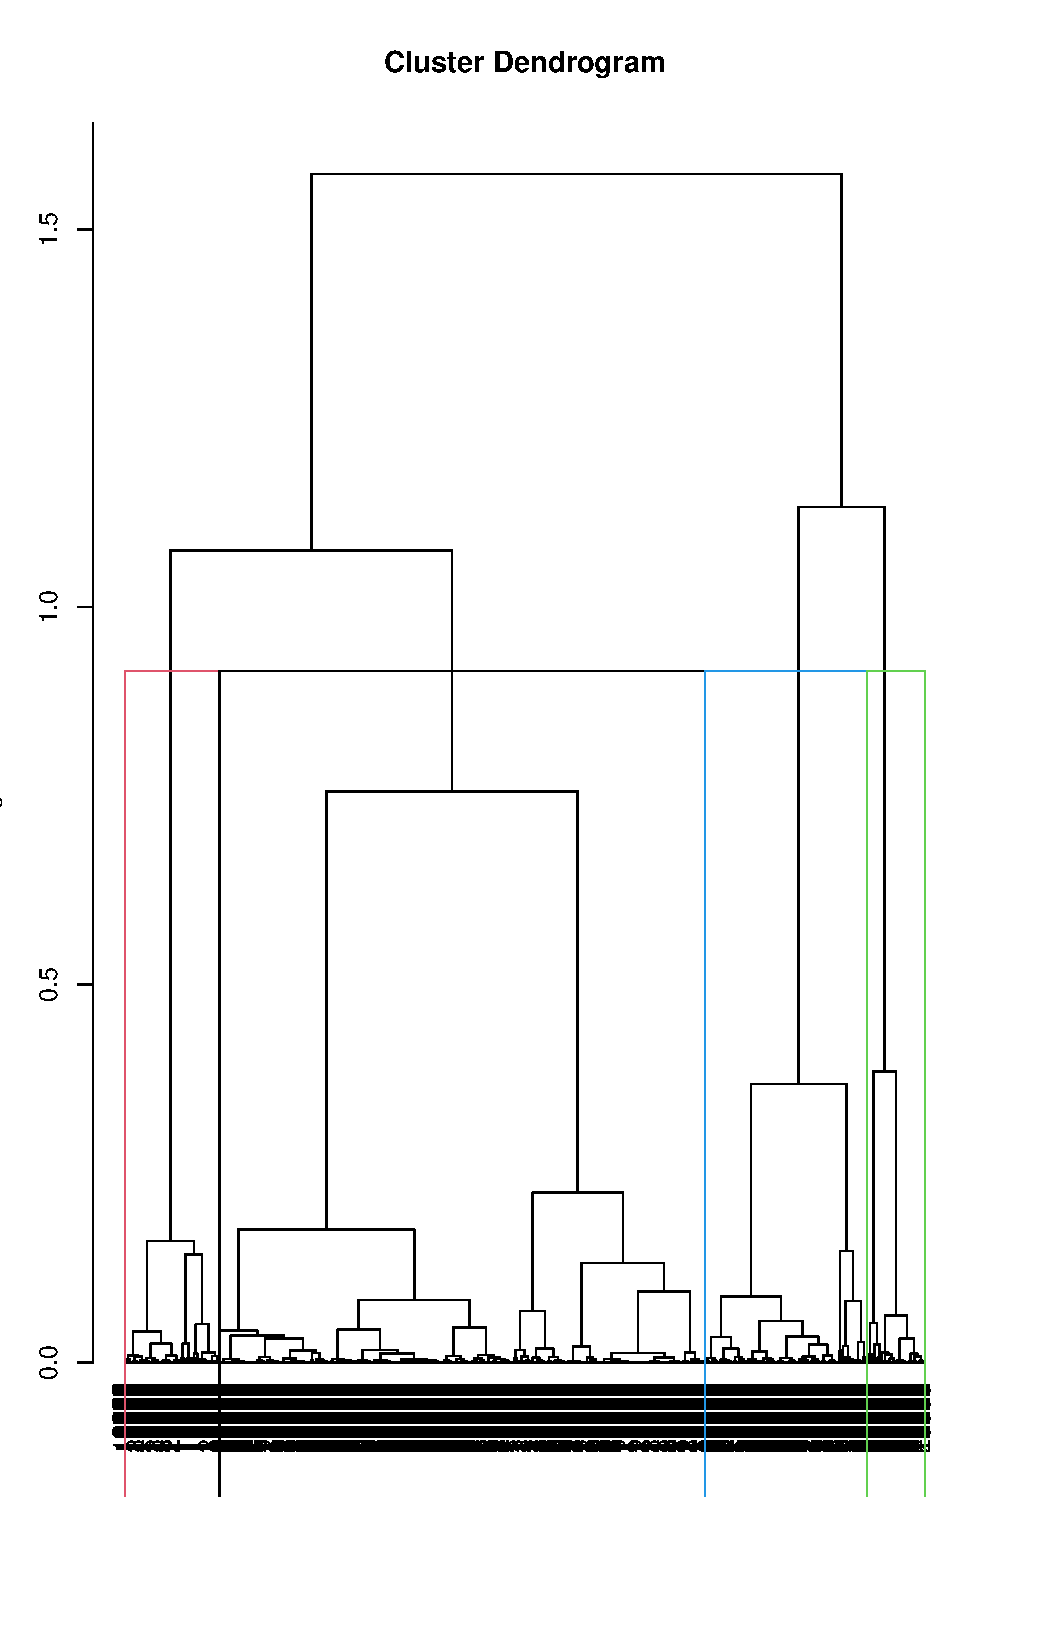
\includegraphics[width=0.8\linewidth]{cluster-dendo-h3}
    \caption{Cluster Dendogram}%
    \label{fig:dendogram-final}
\end{figure}

\end{landscape}


% Discuss about how to get the final number of clusters

\subsection{Description of clusters}%
\label{sub:description_of_clusters}

\begin{table}[h!]
\vspace{5pt}
\caption{Cluster size table}%
\label{tab:cluster_size}
\centering
\begin{subtable}[t]{.3\textwidth}
    \centering
    \caption{Ward cluster size}
    
\begin{tabular}[t]{cr}
\toprule
Cluster & Freq\\
\midrule
1 & 6783\\
2 & 6101\\
3 & 7811\\
\bottomrule
\end{tabular}
\end{subtable}
\begin{subtable}[t]{.3\textwidth}
    \centering
    \caption{HCPC cluster size}
    
\begin{tabular}[t]{lr}
\toprule
c3 & Freq\\
\midrule
1 & 12733\\
2 & 2738\\
3 & 810\\
4 & 4414\\
\bottomrule
\end{tabular}
\end{subtable}
\end{table}


% Table with a description of the clusters size
